\documentclass{scrreprt}
\usepackage[english]{babel}
\usepackage[T1]{fontenc}
\usepackage{lmodern}
\usepackage{blindtext}
\usepackage[utf8]{inputenc}
\usepackage{siunitx} %For unit handling%
\renewcommand{\familydefault}{\sfdefault}
\newcommand{\unit}[1]{\ensuremath{\, \mathrm{#1}}}
\usepackage{amssymb, amsmath, cancel, ulem, graphicx, float, tabularx, multirow, bm}
\usepackage{amsmath}
\usepackage{caption}
\usepackage{subcaption}
\usepackage{tikz}
\newcommand*\circled[1]{\tikz[baseline=(char.base)]{
            \node[shape=circle,draw,inner sep=1pt] (char) {#1};}}
\renewcommand{\phi}{\varphi}

\setcounter{secnumdepth}{5}
\setcounter{tocdepth}{5}

\author{Urs Gerber\\09-921-156 \and Gian-Luca Mateo\\11-113-545}
\date{11th of March 2013}

\title{Lenses}
\subtitle{Practical course report}

\begin{document}

\maketitle

\tableofcontents
\newpage

\chapter{Experiment: Lenses}

\section{Introduction}

\subsection{Goal of the experiment}
The goal of this experiment is to determine the focal distance of a set of lenses using the method proposed by German scientist Friedrich Wilhelm Bessel.

\subsection{Theory}
\subsubsection{Lens equation}
The commonly known lens formula is
\begin{equation}
\frac{1}{f} = \frac{1}{g} + \frac{1}{b}
\end{equation}
where $f$ is the focal distance, $g$ is the object distance and $b$ is the image distance.

\subsubsection{Lense pair}
The lens equation for a pair of lenses $L_1$ and $L_2$ looks a bit different:
\begin{equation}
\frac{1}{f}= \frac{1}{f_1} + \frac{1}{f_2} - \frac{d}{f_1 \cdot f_2}
\end{equation}
where $f_i$ is the focal distance of lense $L_i$ and $d$ is the distance between $L_1$ and $L_2$

\subsubsection{Bessel's method}
We use the method proposed by Bessel to find the focal distance $f$ of a lense by experimental means. Let $a \doteq g + b$ be a fixed quantity. Then there exists for a given focal distance $f < \frac{a}{4}$ only two possible lens positions which produce a sharp image $B$ of object $G$. 

\begin{figure}[H]
	\centering
  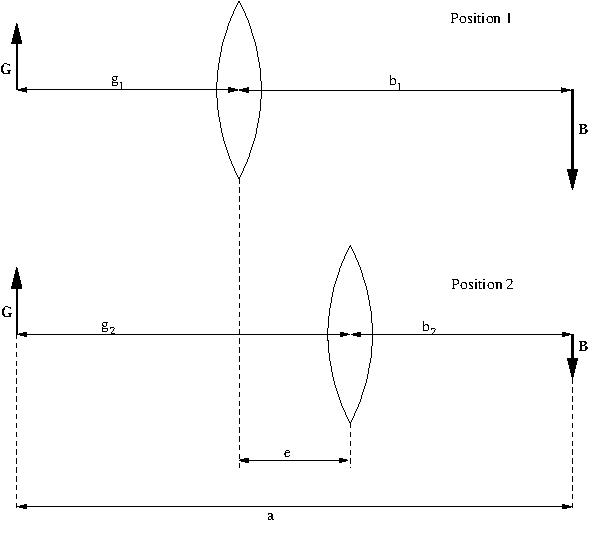
\includegraphics[width=0.9\textwidth]{diag/lens_skript.pdf}
	\caption{Finding focal distance using Bessel's method}
	\label{fig:method}
\end{figure}

These lens positions are given by
\begin{equation}
b_{1,2} = \frac{a}{2} \pm \sqrt{\left(\frac{a}{2}\right)^2-a\cdot f}
\end{equation}

\begin{equation}
g_{1,2} = a-b_{1,2}=b_{2,1} = \frac{a}{2} \mp \sqrt{\left(\frac{a}{2}\right)^2-a\cdot f} 
\end{equation}

\begin{equation}
b_1 - b_2 = 2 \cdot \sqrt{\left(\frac{a}{2}\right)^2-a\cdot f}
\end{equation}

Using $e \doteq b_1 - b_2$ and solving for $f$ yields

\begin{equation}
\boxed{f = \frac{a^2-e^2}{4\cdot a}}
\end{equation}

\section{Experiment setup and execution}

\subsection{Used materials}

\subsection{Assembly}

\section{Measurements}

\section{Analysis and Discussion}

\section{Conclusion}

\begin{thebibliography}{9}

\bibitem{physcript13}
  Peter Wurz,
  \emph{Anleitung zum Physikpraktikum}
  FS2013

\end{thebibliography}

\end{document}
